\noindent

\includegraphics[height=1.25cm]{images/pictograms/benchmark}
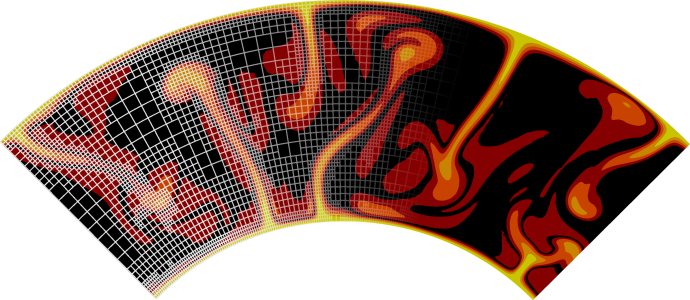
\includegraphics[height=1.25cm]{images/pictograms/aspect_logo}

\includegraphics[height=1.25cm]{images/pictograms/FEM}

\includegraphics[height=1.25cm]{images/pictograms/paraview}


%%%%%%%%%%%%%%%%%%%%%%%%%%%%%%%%%%%%%%%%%%%%%%%%%%%%%%%%%%%%%%%%%%%%%%%%%%%%%%%%%%%%%%%%%%%%%%%%%%%

\begin{flushright} {\tiny {\color{gray} python\_codes/fieldstone\_152/text.tex}} \end{flushright}

\lstinputlisting[language=bash,basicstyle=\small]{python_codes/fieldstone_152/keywords.key}

\par\noindent\rule{\textwidth}{0.4pt}

\begin{center}
\inpython
{\small Code: \url{https://github.com/cedrict/fieldstone/tree/master/python_codes/fieldstone_152}}
\end{center}

\par\noindent\rule{\textwidth}{0.4pt}

%{\sl This stone was developed in collaboration with Donald Duck}. \index{contributors}{D. Duck}

%\par\noindent\rule{\textwidth}{0.4pt}

%%%%%%%%%%%%%%%%%%%%%%%%%%%%%%%%%%%%%%%%%%%%%%%%%%%%%%%%%%%%%%%%%%%%%%%%%%%%%%%%%%%%%%%%%%%%%%%%%%%


The goal here is to explore the influence of the mapping polynomial order and/or
the number of quadrature points on the accuracy of the solution of the so-called 
annulus benchmark (see Section~\ref{MMM-ss:anconv}).

For reference, in this benchmark we solve the Stokes equation for an incompressible
isothermal fluid in an annulus of inner radius $R_1$
and outer radius $R_2$ with the following boundary conditions:
\begin{itemize}
\item Inner boundary: $\upnu_r(R_1,\theta)=0$ 
\item Outer boundary: $\upnu_r(R_2,\theta)=0$ 
\end{itemize}
and the manufactured solution takes the form:
\begin{eqnarray}
\upnu_\theta(r,\theta) &=& f(r) \cos(k\theta) \\
\upnu_r(r,\theta) &=& g(r) k  \sin(k\theta)  \\
p(r,\theta) &=& k h(r) \sin(k \theta) + \rho_0 g_r (r-R_2)  \\
\rho(r,\theta) &=& k \sin (k \theta) \aleph(r) + \rho_0 \\
\end{eqnarray}
with
\begin{eqnarray}
A &=& \frac{2(\ln R_1 - \ln R_2)} { R_2^2 \ln R_1  - R_1^2 \ln R_2}    \nn\\
B &=& \frac{R_2^2-R_1^2}{R_2^2 \ln R_1 - R_1^2 \ln R_2} \nn\\
f(r)   &=& Ar +\frac{B}{r} \nn\\
f'(r)  &=& A - \frac{B}{r^2} \nn\\
g(r)   &=& \frac{A}{2}r  +  \frac{B}{r} \ln r - \frac{1}{r} \nn\\
g'(r)  &=& \frac{A}{2}  +  \frac{B}{r^2} (1-\ln r)   + \frac{1}{r^2} \nn\\
g''(r) &=&  - \frac{B}{r^3} (3 - 2 \ln r )  \nn\\
h(r)   &=& \frac{1}{r^2}(2g-f) \nn\\
\aleph(r) &=&  -g'' - \frac{g'}{r} ( 1 - \frac{2}{r}) + \frac{g}{r^2} (k^2 + 1 -\frac{4}{r})  - \frac{2f}{r^2}  (1-\frac{1}{r}) - \frac{f'}{r^2}   \nn
\end{eqnarray}


\begin{center}
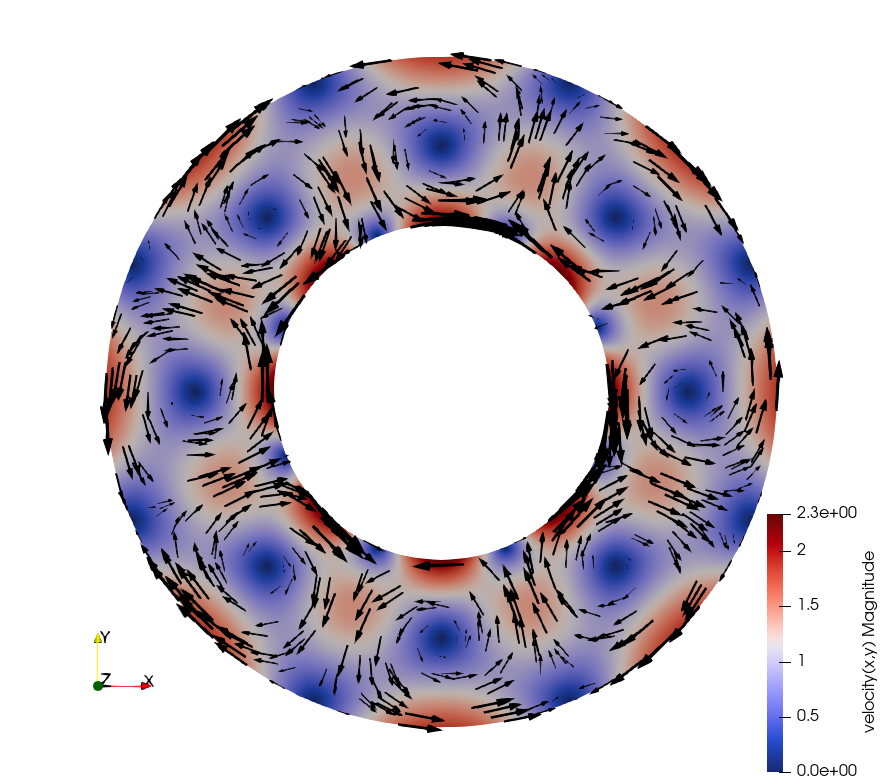
\includegraphics[width=6cm]{python_codes/fieldstone_152/images/vel}
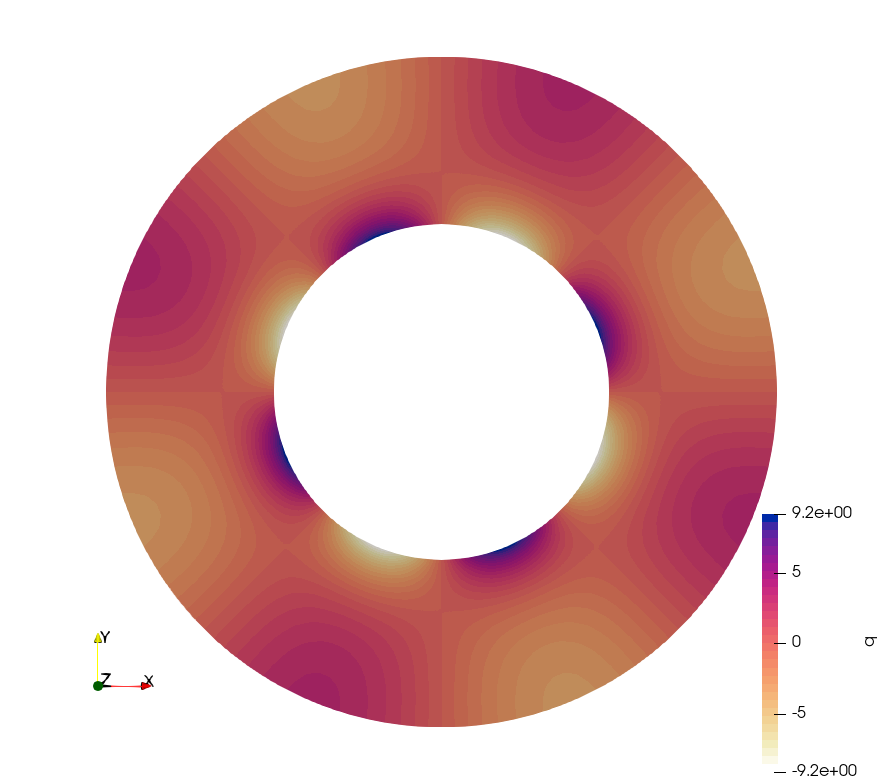
\includegraphics[width=6cm]{python_codes/fieldstone_152/images/press}\\
{\captionfont Velocity and pressure fields for $k=4$.}
\end{center}

\noindent In this \stone we will explore the effect of:
\begin{itemize}
\item resolution via the number of elements in the radial direction: {\python nelr=2-32} (we automatically set {\python nelt=12*nelr})
\item the number of quadrature points per dimension: {\python nqperdim=2,3,4,5}
\item the polynomial order of the mapping: {\python mapping='Q1','Q2','Q3','Q4'}
\end{itemize}
and we will monitor the computed area/volume, the root mean square velocity and the velocity and pressure errors.

After discretising the domain in {\python nel} elements, and having decided the FE
pair we want to use to solve the Stokes equations (in this case \QtwoQone), we end up 
having to compute elemental integrals such as 
\[
\K_e = \int_{\Omega_e} {\bm B}^T\cdot {\bm C}_\eta \cdot {\bm B} \; d\Omega
\]
where $\Omega_e$ denotes an element.
The way we carry out this integration is by means of the Gauss-Legendre quadrature
(see Section~\ref{MMM-sec:quadrature}), which 
forces us to carry out a change of variables from the original element $\Omega_e$ 
to the reference element $(r,s) \in [-1,1]\times [-1,1]$. For this we establish a mapping between both 
as explained in Section~\ref{MMM-ss:mappings}.
Basis functions $Q_{1,2,3,4}$ are defined in Section~\ref{MMM-sec:shpfct2d}.

\begin{center}
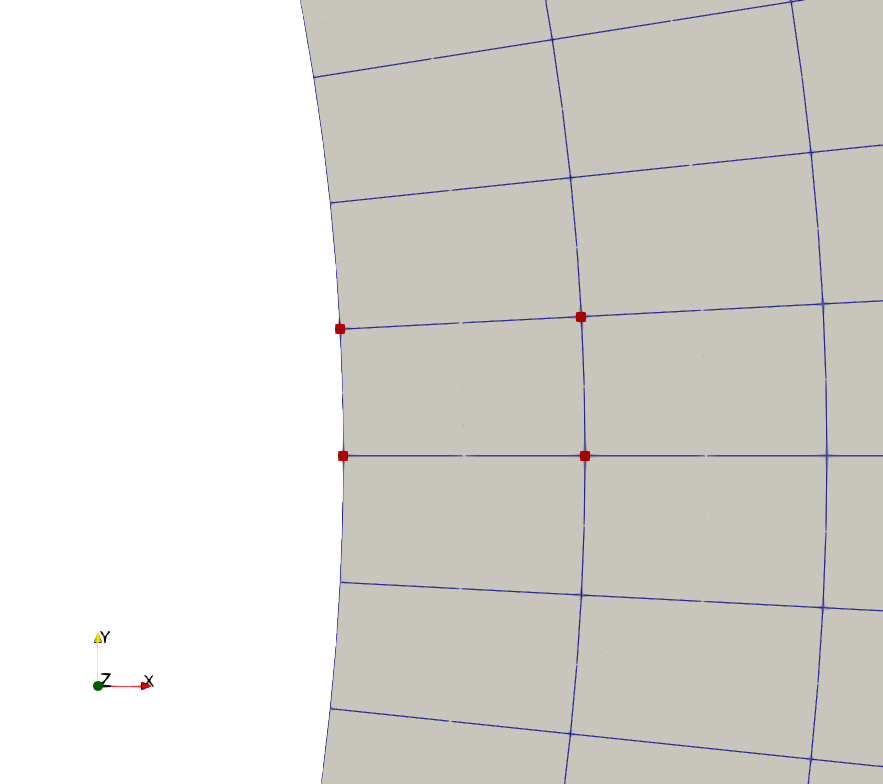
\includegraphics[width=4.2cm]{python_codes/fieldstone_152/images/mappingQ1}
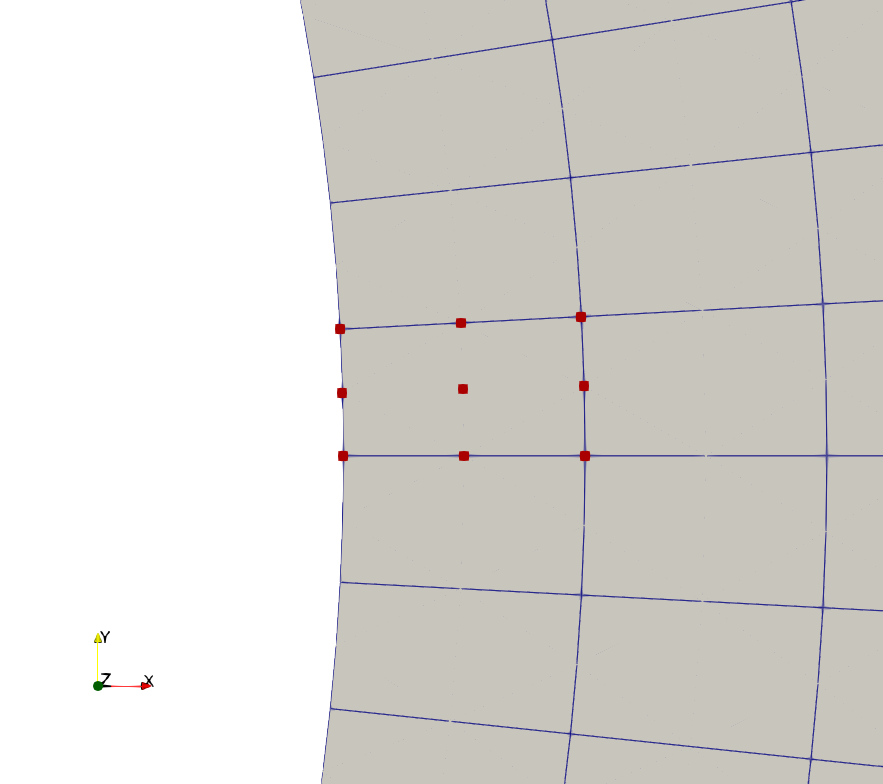
\includegraphics[width=4.2cm]{python_codes/fieldstone_152/images/mappingQ2}
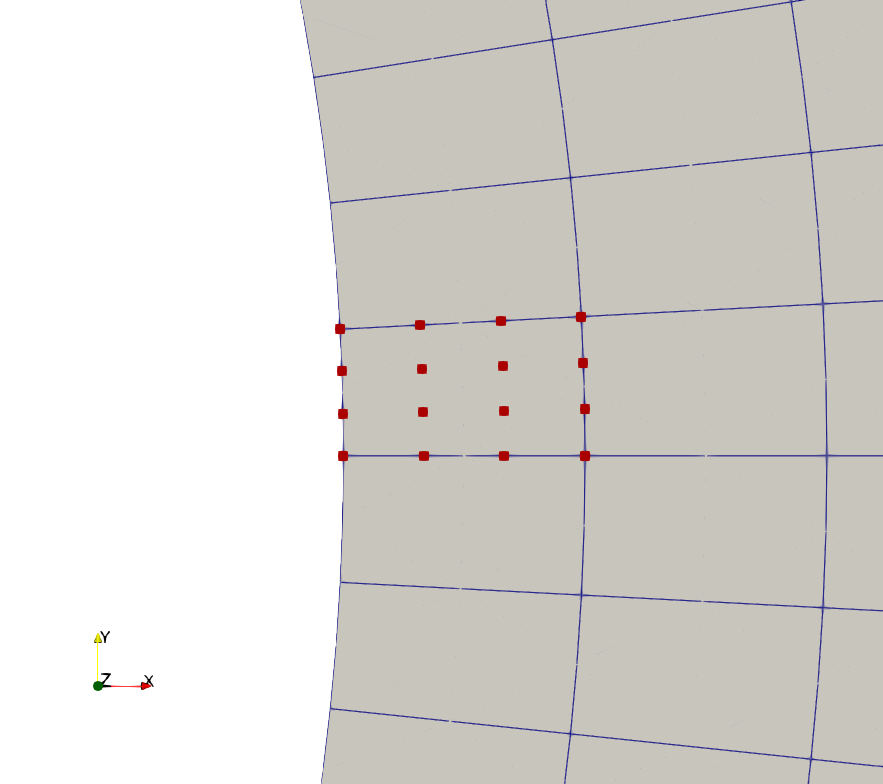
\includegraphics[width=4.2cm]{python_codes/fieldstone_152/images/mappingQ3}
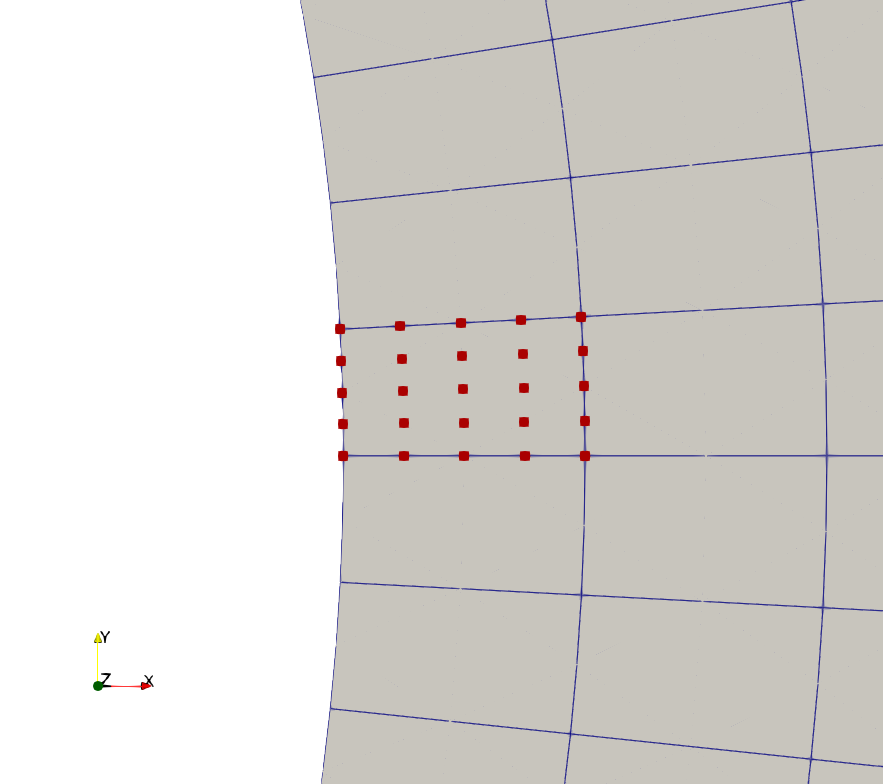
\includegraphics[width=4.2cm]{python_codes/fieldstone_152/images/mappingQ4}\\
{\captionfont Layout of the mapping nodes in element \#0 of the mesh. 
From left to right: $Q_1$, $Q_2$, $Q_3$ and $Q_4$. Rows of nodes are placed 
on concentric circles and columns of nodes are equidistant in $\theta$ space.} 
\end{center}

The code for this \stone is based on \stone~\ref{f21}.  
For each element we store the coordinates of these mapping points into two 
arrays:
\begin{lstlisting}
xmapping=np.zeros((X,nel),dtype=np.float64)
ymapping=np.zeros((X,nel),dtype=np.float64)
\end{lstlisting}
where {\python X} stands for the number of nodes for each mapping.

The reduced coordinates for the quadrature points are given by 
the Gauss-Legendre quadrature approach. The real coordinates of these points
is a function of the mapping used so that 
\begin{lstlisting}
for iel in range(0,nel):
    for kq in range(0,nqel):
        rq=qcoords_r[kq]
        sq=qcoords_s[kq]
        NNNV=NNN(rq,sq,mapping)
        xq=np.dot(NNNV[:],xmapping[:,iel])
        yq=np.dot(NNNV[:],ymapping[:,iel])
\end{lstlisting}
Likewise the Jacobian matrix is by definition a function of the chosen mapping 
so that 
\begin{lstlisting}
for iel in range(0,nel):
    for kq in range(0,nqel):
        rq=qcoords_r[kq]
        sq=qcoords_s[kq]
        dNNNVdr=dNNNdr(rq,sq,mapping)
        dNNNVds=dNNNds(rq,sq,mapping)
        jcb[0,0]=np.dot(dNNNVdr[:],xmapping[:,iel])
        jcb[0,1]=np.dot(dNNNVdr[:],ymapping[:,iel])
        jcb[1,0]=np.dot(dNNNVds[:],xmapping[:,iel])
        jcb[1,1]=np.dot(dNNNVds[:],ymapping[:,iel])
        jcob=np.linalg.det(jcb)
        jcbi=np.linalg.inv(jcb)
\end{lstlisting}


\begin{center}
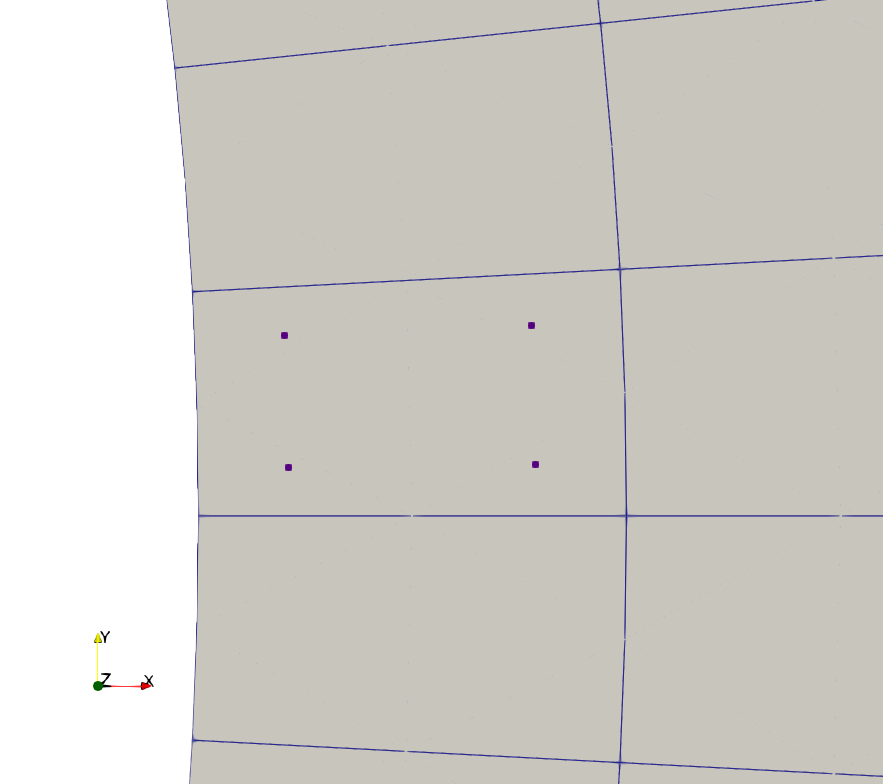
\includegraphics[width=4.2cm]{python_codes/fieldstone_152/images/nq4}
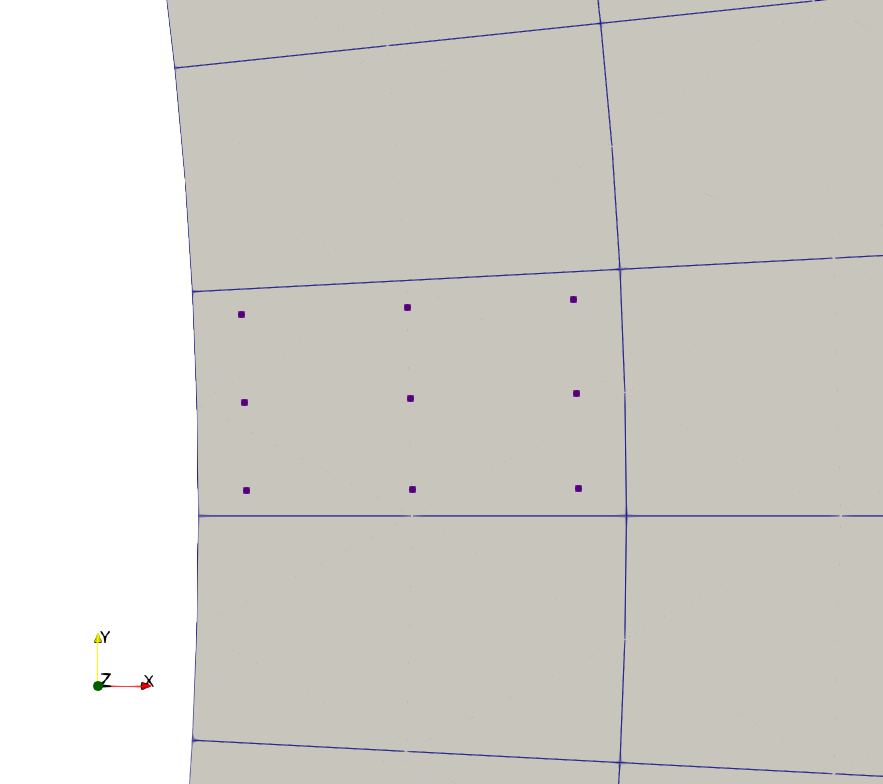
\includegraphics[width=4.2cm]{python_codes/fieldstone_152/images/nq9}
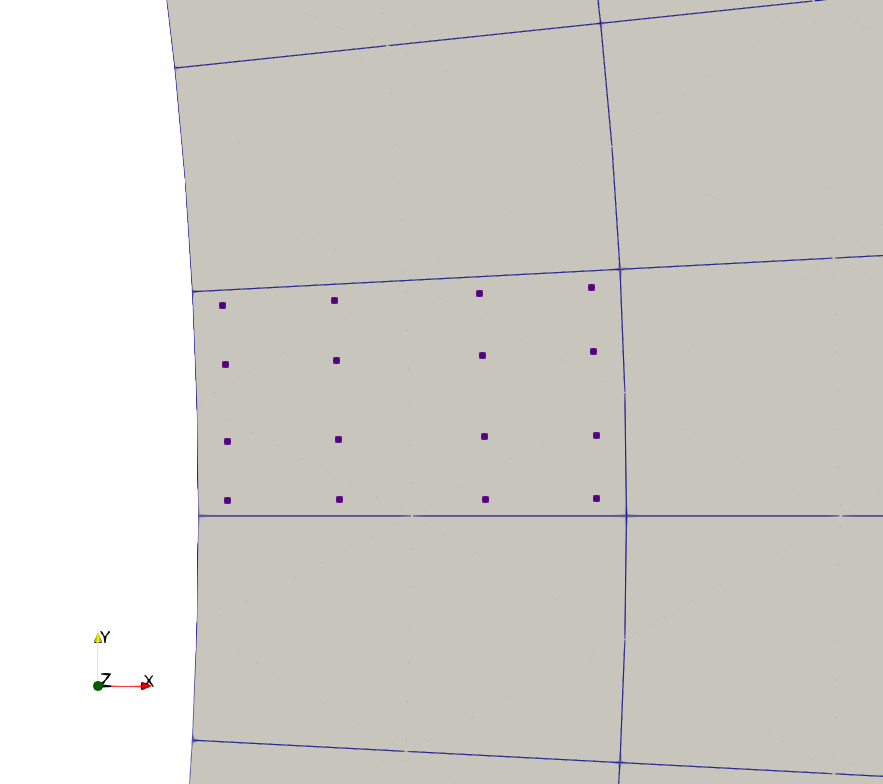
\includegraphics[width=4.2cm]{python_codes/fieldstone_152/images/nq16}
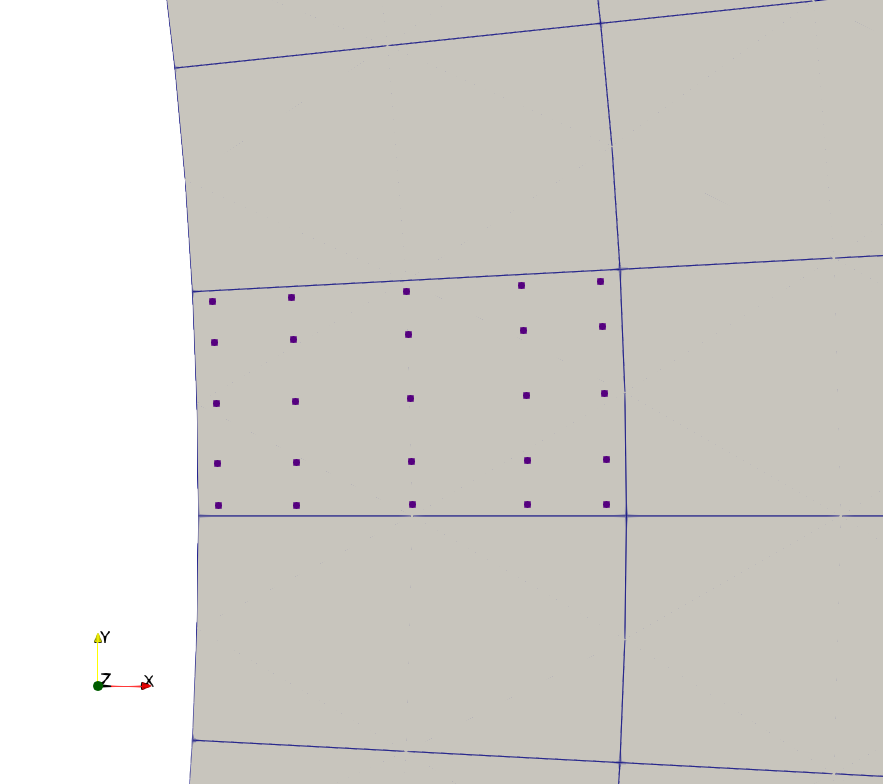
\includegraphics[width=4.2cm]{python_codes/fieldstone_152/images/nq25}\\
{\captionfont Layout of the quadrature points in element \#0 of the mesh. 
From left to right: {\python nqperdim=2,3,4,5}.} 
\end{center}



\newpage
%%%%%%%%%%%%%%%%%%%%%%%%%%%%%%%
\section*{Areas and volumes}

Here we simply compute 
\[
{\cal A} = \sum_e \int_{\Omega_e} d\Omega
\]
where the sum runs over all elements of the annulus
and 
\[
{\cal V} = \sum_e \int_{\Omega_e} 2\pi x d\Omega
\]
for elements on the $x>0$ side of the annulus (axisymmetric formulation)\footnote{the number of elements in the 
tangential direction is a multiple of 4, so element sides always coincide with the $y$-axis.}.
We of course have 
\[
{\cal A}_{analytical} = \pi (R_2^2-R_1^2)
\qquad\qquad
{\cal V}_{analytical} = \frac43 \pi (R_2^3-R_1^3)
\]
so that we can compute the relative errors as a function of resolution, mapping and quadrature: 
\begin{center}
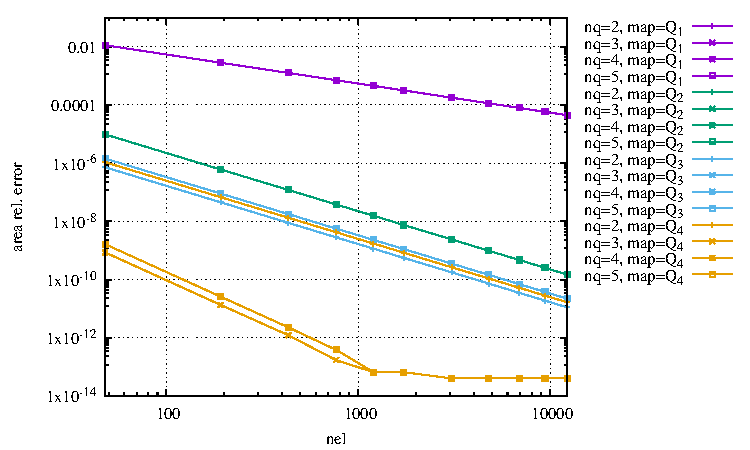
\includegraphics[width=8.3cm]{python_codes/fieldstone_152/results/areas/areas.pdf}
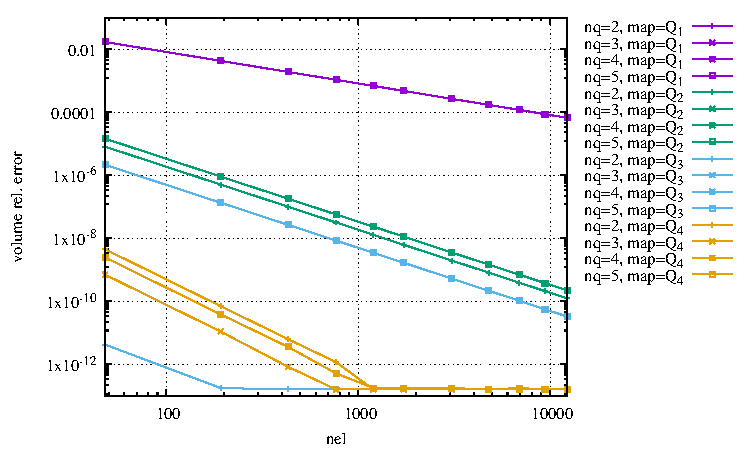
\includegraphics[width=8.3cm]{python_codes/fieldstone_152/results/areas/volumes.pdf}
\end{center}

\noindent Conclusions:
\begin{itemize}
\item unsurprisingly $Q_1$ mapping yields the worst results
\item mapping is the controling factor, much more than quadrature
\item for the isoparametric element (mapping $Q_2$) the number of quadrature points 
is not critical. Results are virtually identical for {\python nqperdim=2,3,4,5}
\item $Q_3$ about one order of magnitude more accurate than $Q_2$ 
\item $Q_4$ mapping 3-4 orders of magnitude more accurate than $Q_2$ mapping
\item I can't explain the {\python nqperdim=2 + mapping=Q3} results that outperform everything else... (volume only)
\end{itemize}

Do these results translate to the solution of the Stokes system? Let's investigate...
The provided {\tt script\_errors} bash script implements a triple loop 
over resolution, number of quadrature points and mapping type.
Results are shown in the following.

\newpage
%%%%%%%%%%%%%%%%%%%%%%%%%%%%%%%%%%%%%%%%%%%%%%%%%%%%%%%%%%%%%%%%%%%%%%%%%%%%%%%%%%%%%
\section*{Annulus convection benchmark (exp=0)}

%---------------------------------------
\subsection*{Root mean square velocity}

\begin{center}
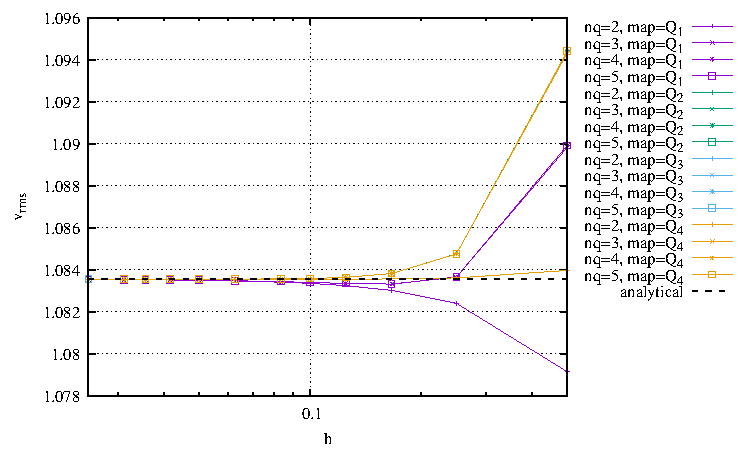
\includegraphics[width=8.3cm]{python_codes/fieldstone_152/results/exp0/vrms}
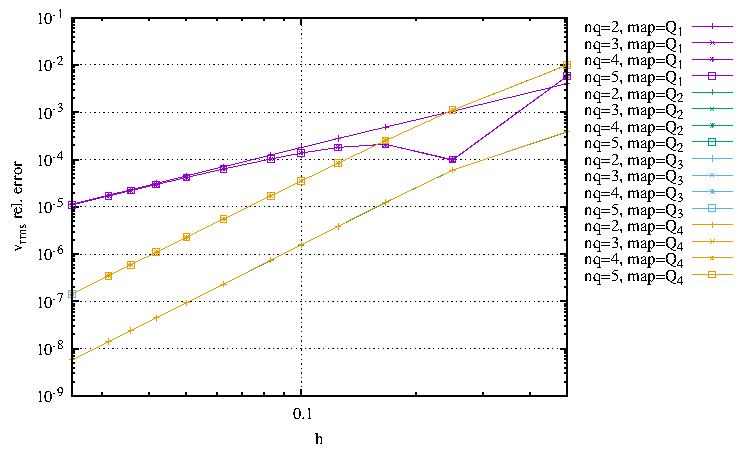
\includegraphics[width=8.3cm]{python_codes/fieldstone_152/results/exp0/vrms_error}\\
{\captionfont Note that we define $h=(R_2-R_1)/nelr=1/nelr$.}
\end{center}

As expected linear mapping yields the worst results. However results are virtually identical for 
the three other mappings.
What is very surprising is the much higher accuracy of {\python nqperdim=2} (i.e. subparametric mapping) ?!


%---------------------------------------
\subsection*{Velocity and pressure errors}

We first look at the min/max values of the nodal velocity and pressure errors over all the nodes:
\begin{center}
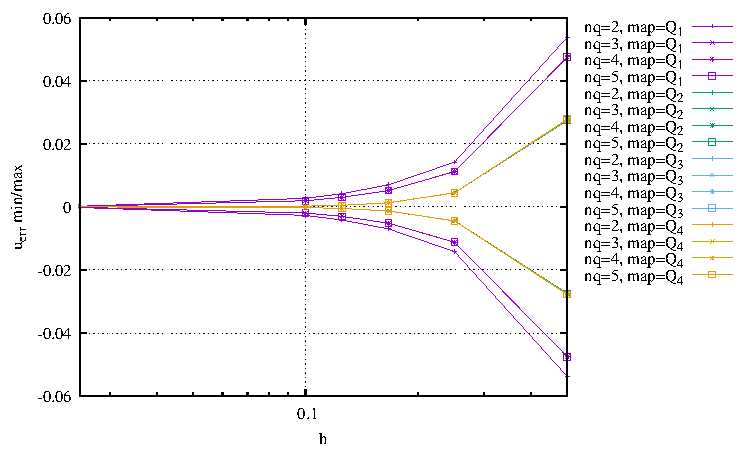
\includegraphics[width=8.3cm]{python_codes/fieldstone_152/results/exp0/u_err}
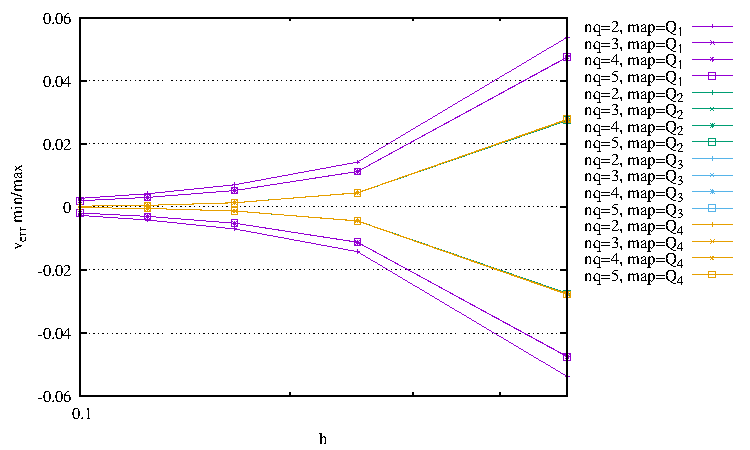
\includegraphics[width=8.3cm]{python_codes/fieldstone_152/results/exp0/v_err}\\
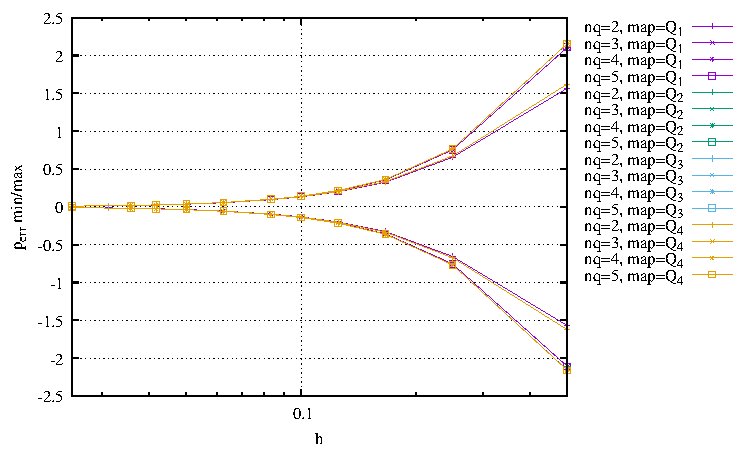
\includegraphics[width=8.3cm]{python_codes/fieldstone_152/results/exp0/p_err}
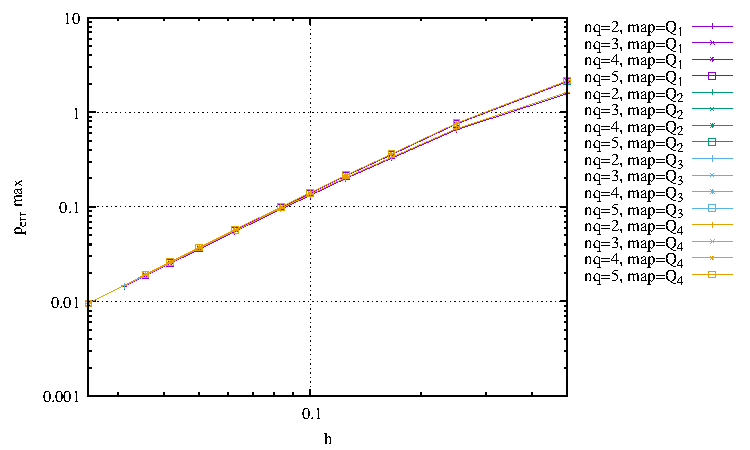
\includegraphics[width=8.3cm]{python_codes/fieldstone_152/results/exp0/p_err_max}\\
{\captionfont Top row: min/max of $u^h(x,y)-u^{th}(x,y)$ and $v^h(x,y)-v^{th}(x,y)$;
Bottom row left: min/max of $p^h(x,y)-p^{th}(x,y)$; bottom row right max of  $p^h(x,y)-p^{th}(x,y)$.} 
\end{center}
We see that all measurements decrease (in amplitude) when the resolution is increased and that 
the $Q_1$ mapping yields the largest errors. 
Interestingly the subparametric case {\python nqperdim=2} seems to yield more accurate 
pressure results.

Turning now to velocity and pressure errors in the $L_2$ norm, 
as expected with the \QtwoQone element (and already shown in \stone~\ref{f21})
we recover a cubic convergence for the velocity error and quadratic for the 
pressure... almost always.

\begin{center}
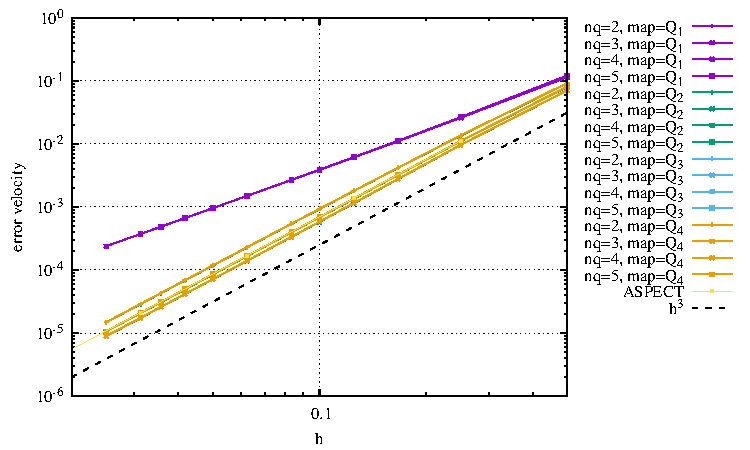
\includegraphics[width=8.3cm]{python_codes/fieldstone_152/results/exp0/errv}
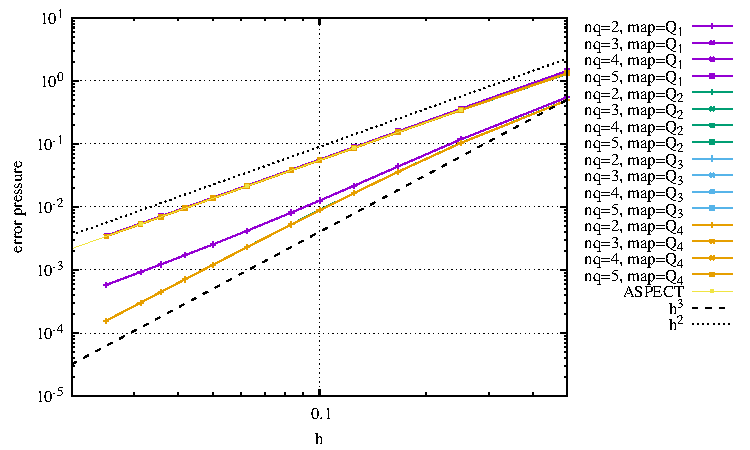
\includegraphics[width=8.3cm]{python_codes/fieldstone_152/results/exp0/errp}
\end{center}

Our velocity and pressure error measurements are identical to those of \aspect.
But why does the subparametric mapping yield a pressure error that is superconvergent?

%IDEA/THOUGHT: are these q points superconvergent points? find ref!

\newpage

%---------------------------------------
\subsection*{Strain rate errors}

Since the analytical velocity field is known so are the strain rate tensor components.
Similarly to \stone~21 this code computes the nodal strain rate components
in three different ways. 
\begin{itemize}
\item method \#1: strain rate components are computed in the middle of the element and then averaged over elements sharing a node.
\item method \#2: strain rate components are computed at each node of the element and then averaged over elements sharing a node.
\item method \#3: global recovery process as documented in Section~\ref{MMM-ss:gradrecovery}.
\end{itemize}

Errors are then computed in the same way as the velocity components.

\begin{center}
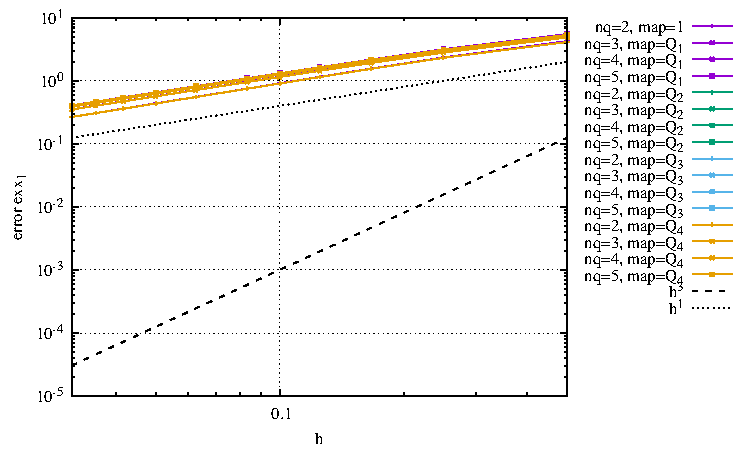
\includegraphics[width=5.7cm]{python_codes/fieldstone_152/results/exp0/err_exx1}
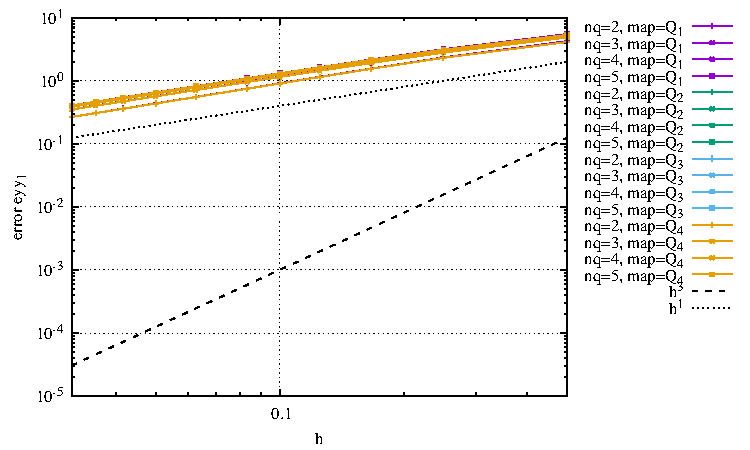
\includegraphics[width=5.7cm]{python_codes/fieldstone_152/results/exp0/err_eyy1}
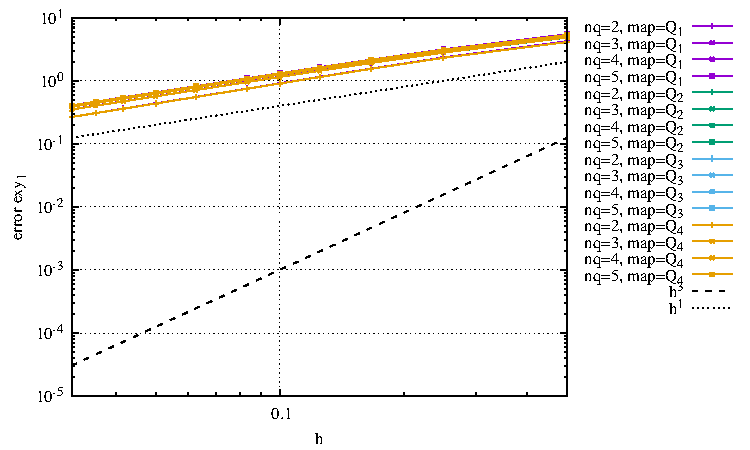
\includegraphics[width=5.7cm]{python_codes/fieldstone_152/results/exp0/err_exy1}\\
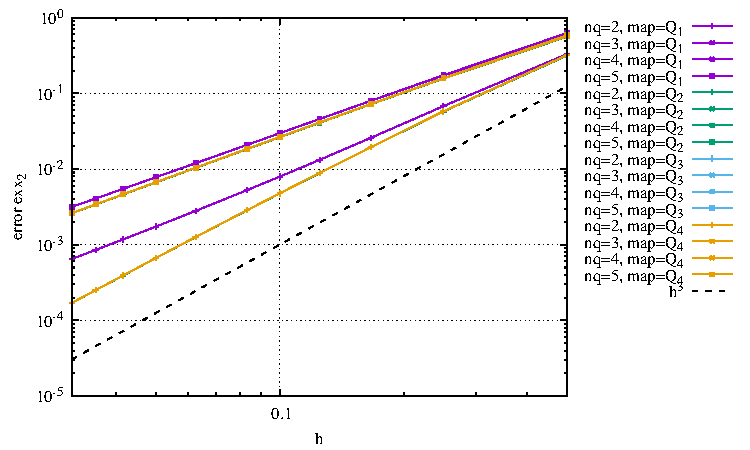
\includegraphics[width=5.7cm]{python_codes/fieldstone_152/results/exp0/err_exx2}
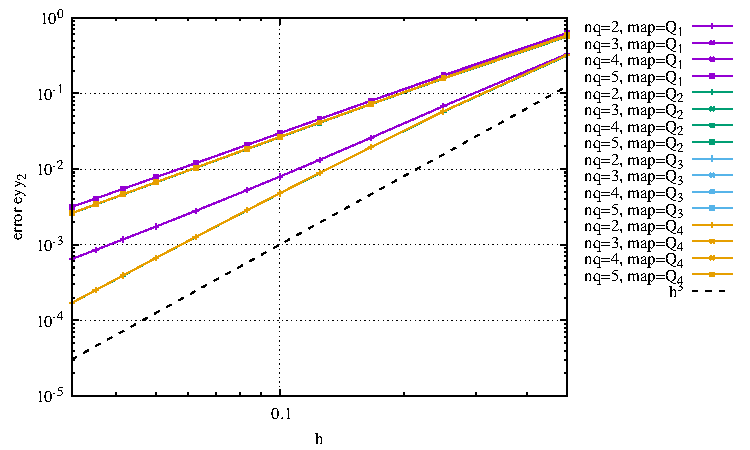
\includegraphics[width=5.7cm]{python_codes/fieldstone_152/results/exp0/err_eyy2}
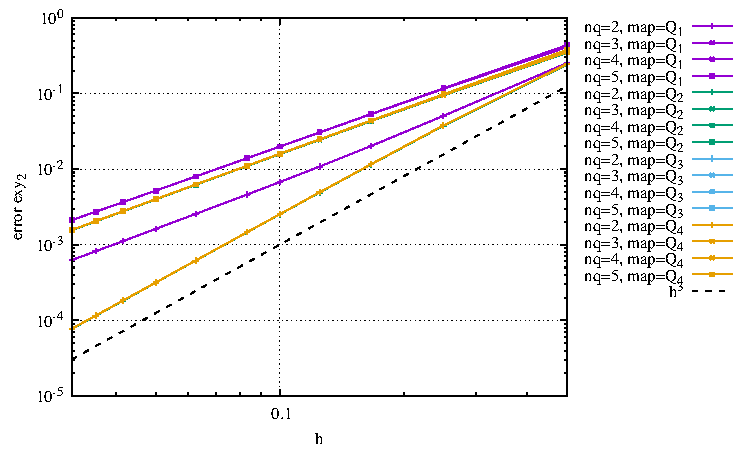
\includegraphics[width=5.7cm]{python_codes/fieldstone_152/results/exp0/err_exy2}\\
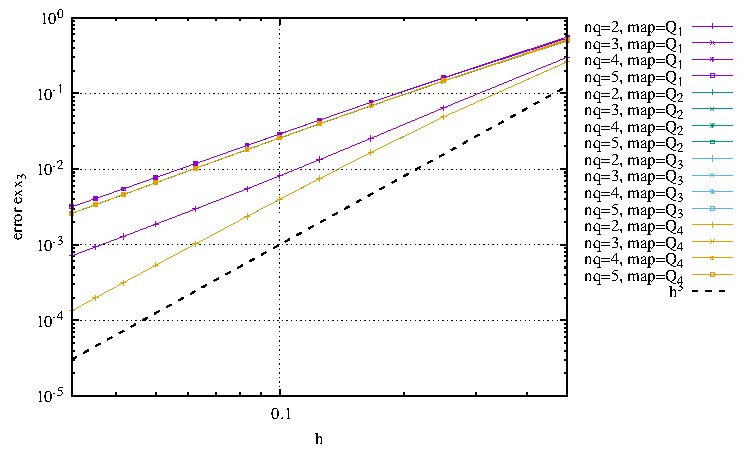
\includegraphics[width=5.7cm]{python_codes/fieldstone_152/results/exp0/err_exx3}
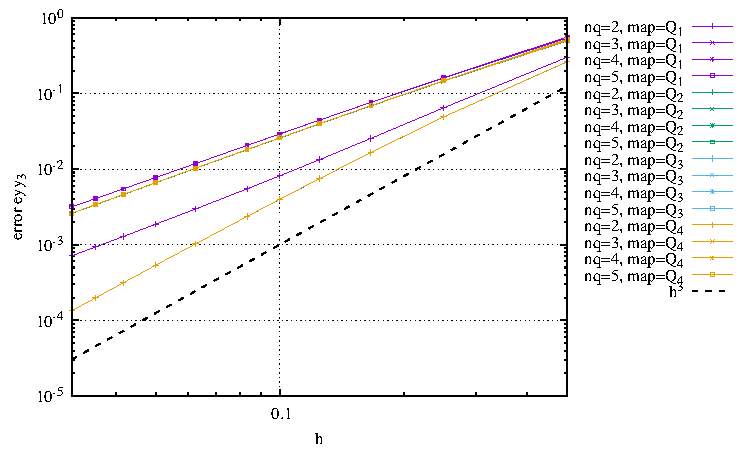
\includegraphics[width=5.7cm]{python_codes/fieldstone_152/results/exp0/err_eyy3}
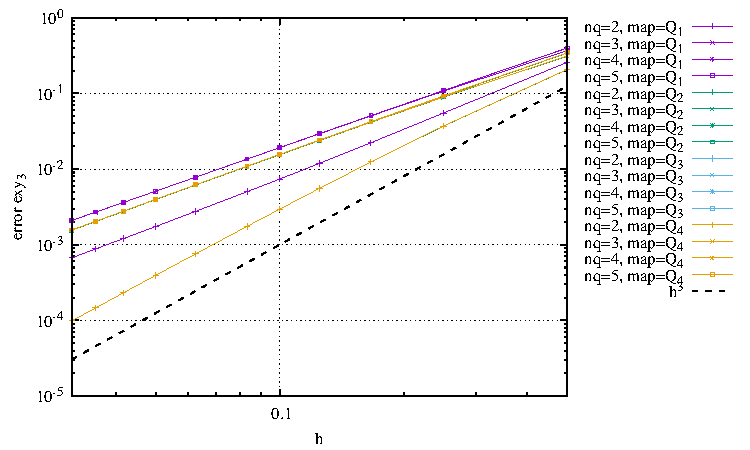
\includegraphics[width=5.7cm]{python_codes/fieldstone_152/results/exp0/err_exy3}
\end{center}

Why the super-convergence for nqperdim=2 ?!?



\newpage
%%%%%%%%%%%%%%%%%%%%%%%%%%%%%%%%%%%%%%%%%%%%%%%%%%%%%%%%%%%%%%%%%%%%%%%%%%%%%%%%%%%%%
\section*{The aquarium test (exp=1) - plane strain}

obtained with 8 elements in radial direction

\begin{center}
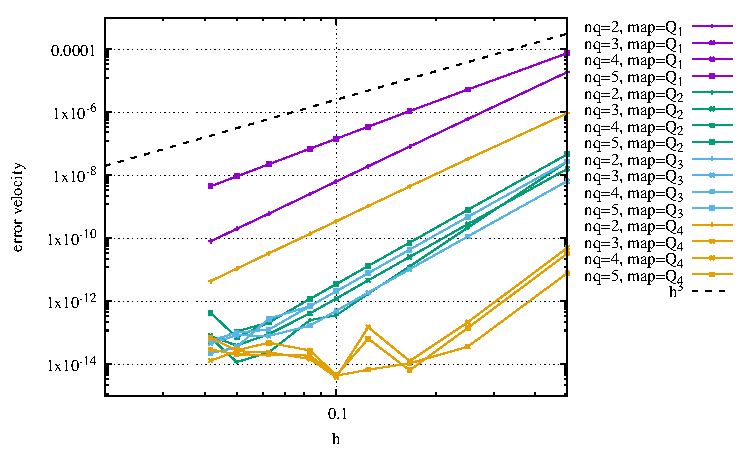
\includegraphics[width=8.3cm]{python_codes/fieldstone_152/results/exp1/errv}
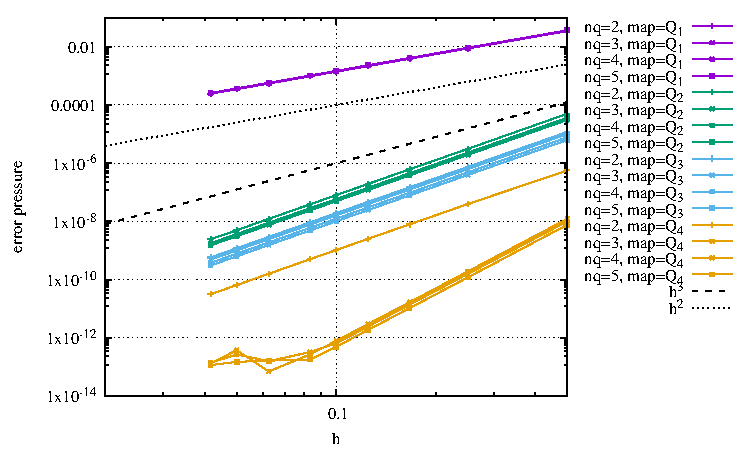
\includegraphics[width=8.3cm]{python_codes/fieldstone_152/results/exp1/errp}
\end{center}

\begin{center}
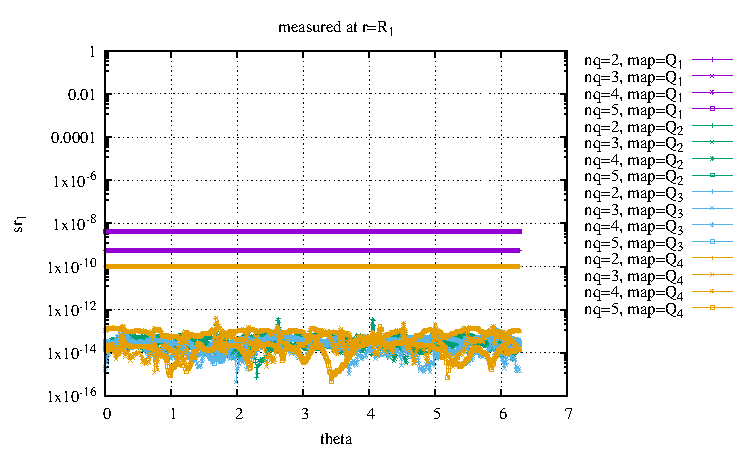
\includegraphics[width=5.7cm]{python_codes/fieldstone_152/results/exp1/sr1_R1}
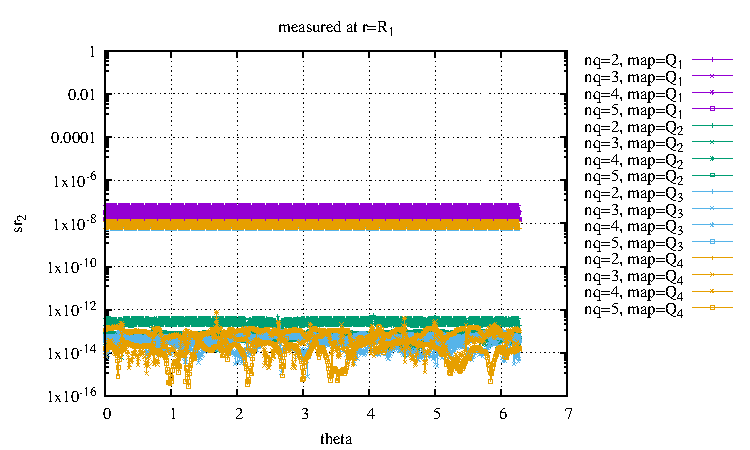
\includegraphics[width=5.7cm]{python_codes/fieldstone_152/results/exp1/sr2_R1}
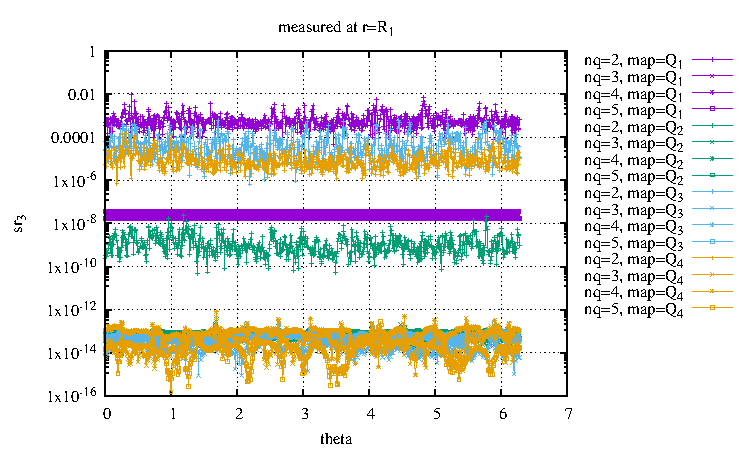
\includegraphics[width=5.7cm]{python_codes/fieldstone_152/results/exp1/sr3_R1}\\
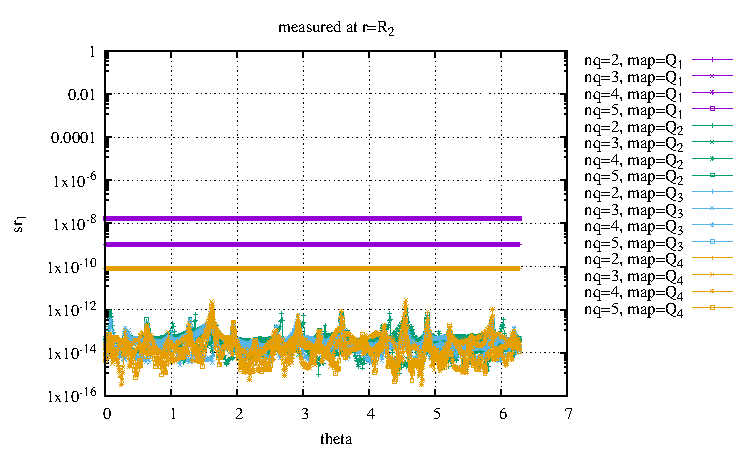
\includegraphics[width=5.7cm]{python_codes/fieldstone_152/results/exp1/sr1_R2}
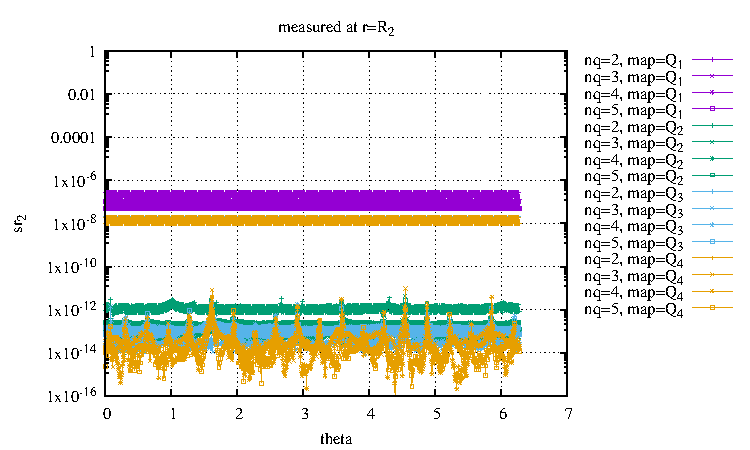
\includegraphics[width=5.7cm]{python_codes/fieldstone_152/results/exp1/sr2_R2}
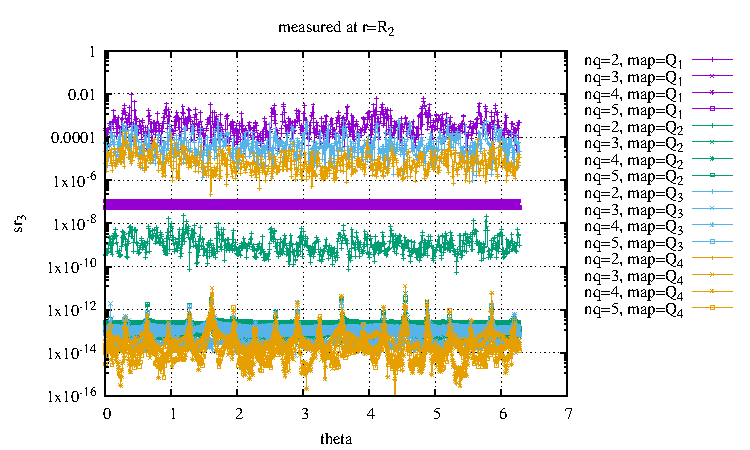
\includegraphics[width=5.7cm]{python_codes/fieldstone_152/results/exp1/sr3_R2}\\
\end{center}

\begin{center}
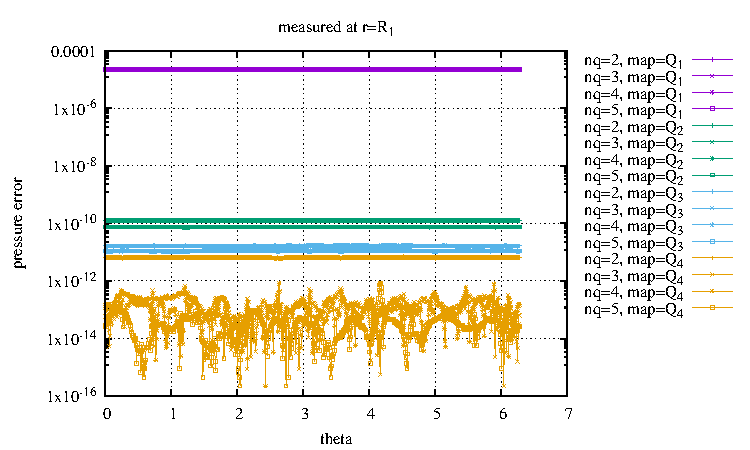
\includegraphics[width=8.3cm]{python_codes/fieldstone_152/results/exp1/qqq_R1}
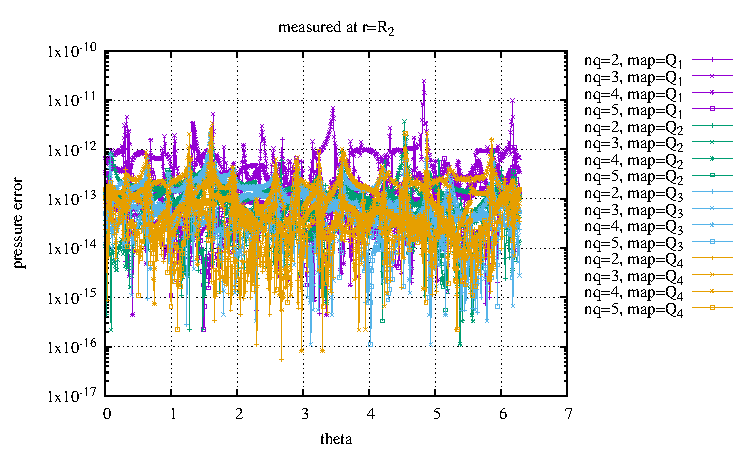
\includegraphics[width=8.3cm]{python_codes/fieldstone_152/results/exp1/qqq_R2}
\end{center}


\newpage
%%%%%%%%%%%%%%%%%%%%%%%%%%%%%%%%%%%%%%%%%%%%%%%%%%%%%%%%%%%%%%%%%%%%%%%%%%%%%%%%%%%%%
\section*{The aquarium test (exp=1) - axisymmetric}

obtained with 8 elements in radial direction

\begin{center}
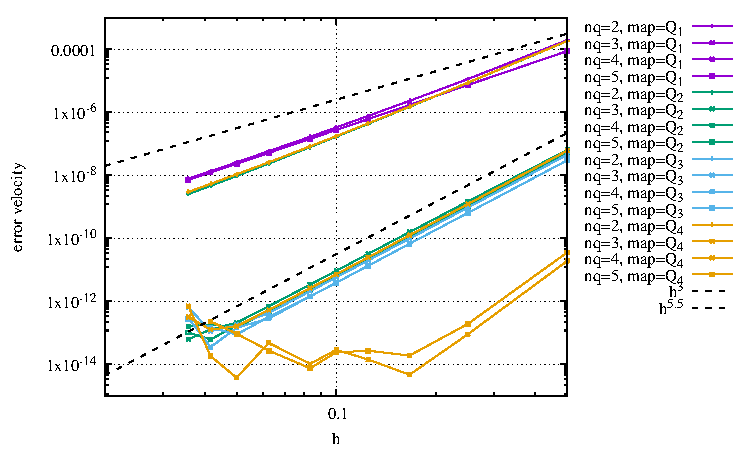
\includegraphics[width=8.3cm]{python_codes/fieldstone_152/results/exp1_axisymmetric/errv}
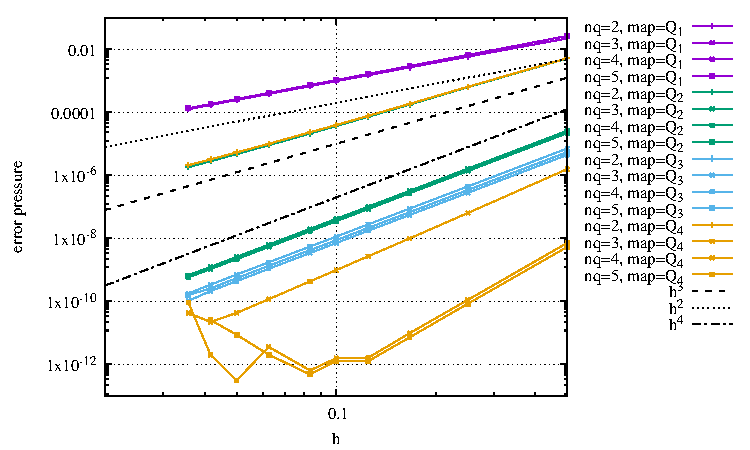
\includegraphics[width=8.3cm]{python_codes/fieldstone_152/results/exp1_axisymmetric/errp}
\end{center}


\begin{center}
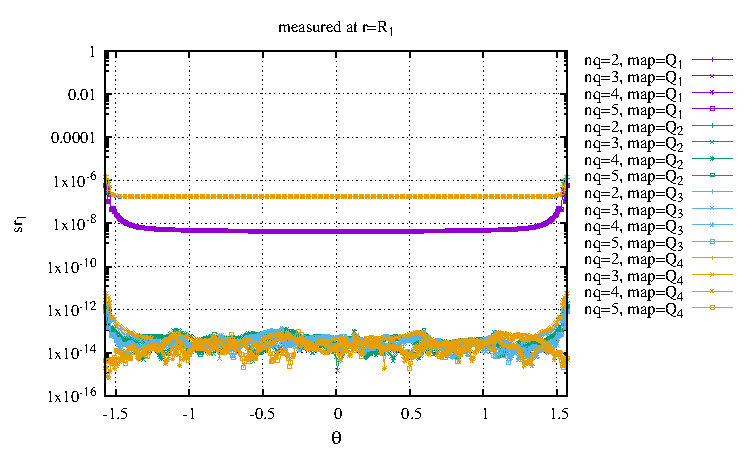
\includegraphics[width=5.7cm]{python_codes/fieldstone_152/results/exp1_axisymmetric/sr1_R1}
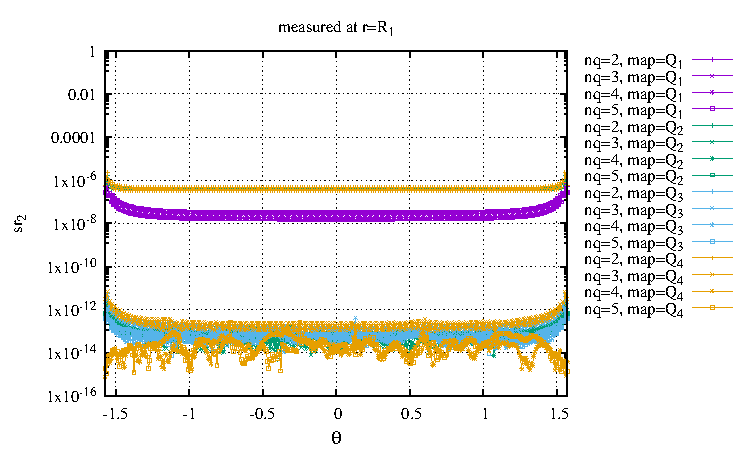
\includegraphics[width=5.7cm]{python_codes/fieldstone_152/results/exp1_axisymmetric/sr2_R1}
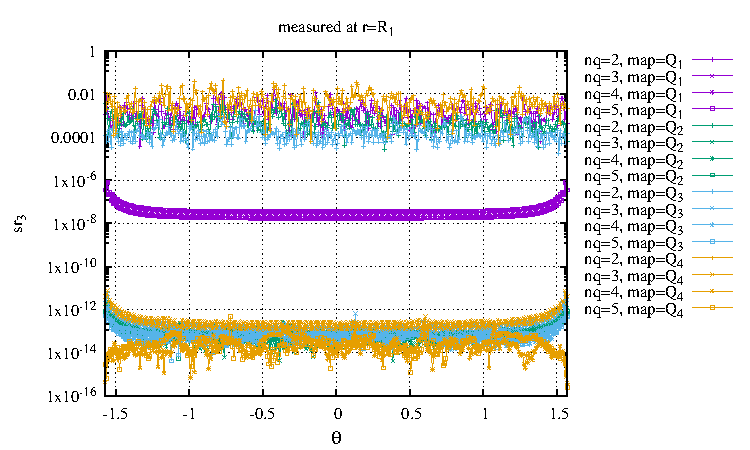
\includegraphics[width=5.7cm]{python_codes/fieldstone_152/results/exp1_axisymmetric/sr3_R1}\\
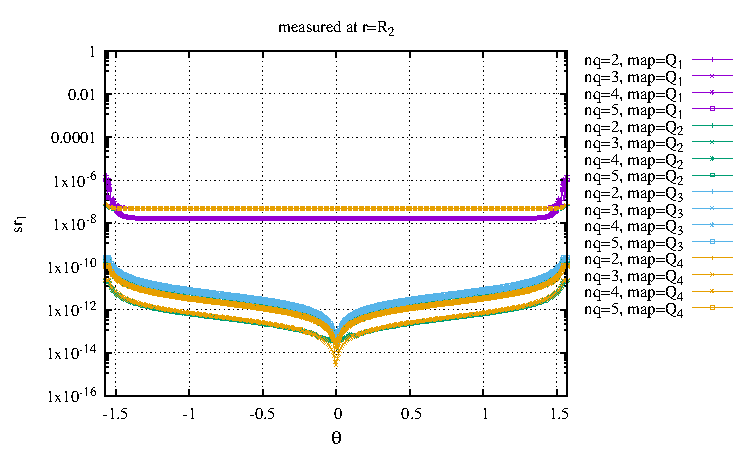
\includegraphics[width=5.7cm]{python_codes/fieldstone_152/results/exp1_axisymmetric/sr1_R2}
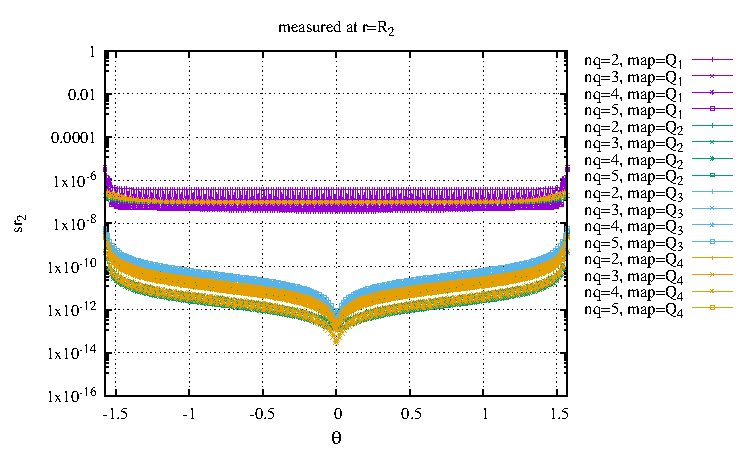
\includegraphics[width=5.7cm]{python_codes/fieldstone_152/results/exp1_axisymmetric/sr2_R2}
\includegraphics[width=5.7cm]{python_codes/fieldstone_152/results/exp1_axisymmetric/sr3_R2}\\
\end{center}


\begin{center}
\includegraphics[width=8.3cm]{python_codes/fieldstone_152/results/exp1_axisymmetric/qqq_R1}
\includegraphics[width=8.3cm]{python_codes/fieldstone_152/results/exp1_axisymmetric/qqq_R2}
\end{center}

Conclusion: best/cheapest results obtained for nqperdim=4 and Q4



\newpage
%%%%%%%%%%%%%%%%%%%%%%%%%%%%%%%%%%%%%%%%%%%%%%%%%%%%%%%%%%%%%%%%%%%%%%%%%%%%%%%%%%%%%
\section*{The blob test (exp=2) - plane strain}

obtained with 8 elements in radial direction - {\tt script\_sr}

\begin{center}
\includegraphics[width=5.7cm]{python_codes/fieldstone_152/results/exp2/sr1_R1}
\includegraphics[width=5.7cm]{python_codes/fieldstone_152/results/exp2/sr2_R1}
\includegraphics[width=5.7cm]{python_codes/fieldstone_152/results/exp2/sr3_R1}\\
\includegraphics[width=5.7cm]{python_codes/fieldstone_152/results/exp2/sr1_R2}
\includegraphics[width=5.7cm]{python_codes/fieldstone_152/results/exp2/sr2_R2}
\includegraphics[width=5.7cm]{python_codes/fieldstone_152/results/exp2/sr3_R2}\\
\end{center}

\begin{center}
\includegraphics[width=8.3cm]{python_codes/fieldstone_152/results/exp2/qqq_R1}
\includegraphics[width=8.3cm]{python_codes/fieldstone_152/results/exp2/qqq_R2}
\end{center}

\newpage
%%%%%%%%%%%%%%%%%%%%%%%%%%%%%%%%%%%%%%%%%%%%%%%%%%%%%%%%%%%%%%%%%%%%%%%%%%%%%%%%%%%%%
\section*{The blob test (exp=2) - axisymmetric}

obtained with 8 elements in radial direction

\begin{center}
\includegraphics[width=5.7cm]{python_codes/fieldstone_152/results/exp2_axisymmetric/nelr_08/sr1_R1}
\includegraphics[width=5.7cm]{python_codes/fieldstone_152/results/exp2_axisymmetric/nelr_08/sr2_R1}
\includegraphics[width=5.7cm]{python_codes/fieldstone_152/results/exp2_axisymmetric/nelr_08/sr3_R1}\\
\includegraphics[width=5.7cm]{python_codes/fieldstone_152/results/exp2_axisymmetric/nelr_08/sr1_R2}
\includegraphics[width=5.7cm]{python_codes/fieldstone_152/results/exp2_axisymmetric/nelr_08/sr2_R2}
\includegraphics[width=5.7cm]{python_codes/fieldstone_152/results/exp2_axisymmetric/nelr_08/sr3_R2}\\
\end{center}

\begin{center}
\includegraphics[width=8.3cm]{python_codes/fieldstone_152/results/exp2_axisymmetric/nelr_08/qqq_R1}
\includegraphics[width=8.3cm]{python_codes/fieldstone_152/results/exp2_axisymmetric/nelr_08/qqq_R2}
\end{center}

\newpage

obtained with 16 elements in radial direction, Q1 mapping data removed for readability

\begin{center}
\includegraphics[width=5.7cm]{python_codes/fieldstone_152/results/exp2_axisymmetric/nelr_16/sr1_R1}
\includegraphics[width=5.7cm]{python_codes/fieldstone_152/results/exp2_axisymmetric/nelr_16/sr2_R1}
\includegraphics[width=5.7cm]{python_codes/fieldstone_152/results/exp2_axisymmetric/nelr_16/sr3_R1}\\
\includegraphics[width=5.7cm]{python_codes/fieldstone_152/results/exp2_axisymmetric/nelr_16/sr1_R2}
\includegraphics[width=5.7cm]{python_codes/fieldstone_152/results/exp2_axisymmetric/nelr_16/sr2_R2}
\includegraphics[width=5.7cm]{python_codes/fieldstone_152/results/exp2_axisymmetric/nelr_16/sr3_R2}\\
\end{center}

\begin{center}
\includegraphics[width=8.3cm]{python_codes/fieldstone_152/results/exp2_axisymmetric/nelr_16/qqq_R1}
\includegraphics[width=8.3cm]{python_codes/fieldstone_152/results/exp2_axisymmetric/nelr_16/qqq_R2}
\end{center}

obvious conclusion is nqperdim=2 not fine.

\newpage

obtained with 24 elements in radial direction, Q1 mapping data and nqperdim=2 data removed for readability

\begin{center}
\includegraphics[width=5.7cm]{python_codes/fieldstone_152/results/exp2_axisymmetric/nelr_24/sr1_R1}
\includegraphics[width=5.7cm]{python_codes/fieldstone_152/results/exp2_axisymmetric/nelr_24/sr2_R1}
\includegraphics[width=5.7cm]{python_codes/fieldstone_152/results/exp2_axisymmetric/nelr_24/sr3_R1}\\
\includegraphics[width=5.7cm]{python_codes/fieldstone_152/results/exp2_axisymmetric/nelr_24/sr1_R2}
\includegraphics[width=5.7cm]{python_codes/fieldstone_152/results/exp2_axisymmetric/nelr_24/sr2_R2}
\includegraphics[width=5.7cm]{python_codes/fieldstone_152/results/exp2_axisymmetric/nelr_24/sr3_R2}\\
\end{center}

\begin{center}
\includegraphics[width=8.3cm]{python_codes/fieldstone_152/results/exp2_axisymmetric/nelr_24/qqq_R1}
\includegraphics[width=8.3cm]{python_codes/fieldstone_152/results/exp2_axisymmetric/nelr_24/qqq_R2}
\end{center}

\newpage

obtained with 32 elements in radial direction, Q1 mapping data and nqperdim=2 data removed for readability
point size decreased.

\begin{center}
\includegraphics[width=5.7cm]{python_codes/fieldstone_152/results/exp2_axisymmetric/nelr_32/sr1_R1}
\includegraphics[width=5.7cm]{python_codes/fieldstone_152/results/exp2_axisymmetric/nelr_32/sr2_R1}
\includegraphics[width=5.7cm]{python_codes/fieldstone_152/results/exp2_axisymmetric/nelr_32/sr3_R1}\\
\includegraphics[width=5.7cm]{python_codes/fieldstone_152/results/exp2_axisymmetric/nelr_32/sr1_R2}
\includegraphics[width=5.7cm]{python_codes/fieldstone_152/results/exp2_axisymmetric/nelr_32/sr2_R2}
\includegraphics[width=5.7cm]{python_codes/fieldstone_152/results/exp2_axisymmetric/nelr_32/sr3_R2}\\
\end{center}

\begin{center}
\includegraphics[width=8.3cm]{python_codes/fieldstone_152/results/exp2_axisymmetric/nelr_32/qqq_R1}
\includegraphics[width=8.3cm]{python_codes/fieldstone_152/results/exp2_axisymmetric/nelr_32/qqq_R2}
\end{center}

Run with ASPECT and plot against these

\newpage


\begin{center}
\includegraphics[width=8.3cm]{python_codes/fieldstone_152/results/exp2_axisymmetric/rho}
\includegraphics[width=8.3cm]{python_codes/fieldstone_152/results/exp2_axisymmetric/vel}\\
\includegraphics[width=8.3cm]{python_codes/fieldstone_152/results/exp2_axisymmetric/press}
\includegraphics[width=8.3cm]{python_codes/fieldstone_152/results/exp2_axisymmetric/sr}\\
{\captionfont nelr=32, nqperdim=3, Q4 mapping.} 
\end{center}



\newpage
%%%%%%%%%%%%%%%%%%%%%%%%%%%%%%%%%%%%%%%%%%%%%%%%%%%%%%%%%%%%%%%%%%%%%%%%%%%%%%%%%%%%%
\section*{The blob test (exp=2) - axisymmetric + free slip}

obtained with 8 elements in radial direction

\begin{center}
\includegraphics[width=5.7cm]{python_codes/fieldstone_152/results/exp2_axisymmetric_fs/nelr_08/sr1_R1}
\includegraphics[width=5.7cm]{python_codes/fieldstone_152/results/exp2_axisymmetric_fs/nelr_08/sr2_R1}
\includegraphics[width=5.7cm]{python_codes/fieldstone_152/results/exp2_axisymmetric_fs/nelr_08/sr3_R1}\\
\includegraphics[width=5.7cm]{python_codes/fieldstone_152/results/exp2_axisymmetric_fs/nelr_08/sr1_R2}
\includegraphics[width=5.7cm]{python_codes/fieldstone_152/results/exp2_axisymmetric_fs/nelr_08/sr2_R2}
\includegraphics[width=5.7cm]{python_codes/fieldstone_152/results/exp2_axisymmetric_fs/nelr_08/sr3_R2}\\
\end{center}

\begin{center}
\includegraphics[width=8.3cm]{python_codes/fieldstone_152/results/exp2_axisymmetric_fs/nelr_08/qqq_R1}
\includegraphics[width=8.3cm]{python_codes/fieldstone_152/results/exp2_axisymmetric_fs/nelr_08/qqq_R2}
\end{center}

\begin{center}
\includegraphics[width=8.3cm]{python_codes/fieldstone_152/results/exp2_axisymmetric_fs/nelr_08/vt_R2}
\includegraphics[width=8.3cm]{python_codes/fieldstone_152/results/exp2_axisymmetric_fs/nelr_08/err_R2}
\end{center}

Run with ASPECT and plot against these





\newpage
obtained with 32 elements in radial direction, Q1 mapping data and nqperdim=2 data removed for readability
point size decreased.

\begin{center}
\includegraphics[width=5.7cm]{python_codes/fieldstone_152/results/exp2_axisymmetric_fs/nelr_32/sr1_R1}
\includegraphics[width=5.7cm]{python_codes/fieldstone_152/results/exp2_axisymmetric_fs/nelr_32/sr2_R1}
\includegraphics[width=5.7cm]{python_codes/fieldstone_152/results/exp2_axisymmetric_fs/nelr_32/sr3_R1}\\
\includegraphics[width=5.7cm]{python_codes/fieldstone_152/results/exp2_axisymmetric_fs/nelr_32/sr1_R2}
\includegraphics[width=5.7cm]{python_codes/fieldstone_152/results/exp2_axisymmetric_fs/nelr_32/sr2_R2}
\includegraphics[width=5.7cm]{python_codes/fieldstone_152/results/exp2_axisymmetric_fs/nelr_32/sr3_R2}\\
\end{center}

\begin{center}
\includegraphics[width=8.3cm]{python_codes/fieldstone_152/results/exp2_axisymmetric_fs/nelr_32/qqq_R1}
\includegraphics[width=8.3cm]{python_codes/fieldstone_152/results/exp2_axisymmetric_fs/nelr_32/qqq_R2}
\end{center}

\begin{center}
\includegraphics[width=8.3cm]{python_codes/fieldstone_152/results/exp2_axisymmetric_fs/nelr_32/vt_R2}
\includegraphics[width=8.3cm]{python_codes/fieldstone_152/results/exp2_axisymmetric_fs/nelr_32/err_R2}
\end{center}


THERE REMAINS a pb: strain rate far away from blob should go to zero. It was the case with no-slip!

look at olga stuff about normals and jacobian?1

Run with ASPECT and plot against these


















\newpage
%%%%%%%%%%%%%%%%%%%%%%%%%%%%%%%%%%%%%%%%%%%%%%%%%%%%%%%%%%%%%%%%%%%%%%%%%%%%%%%%%%%%%%%%%%%%%%%%%%%
\par\noindent\rule{\textwidth}{0.4pt}

\vspace{.5cm}

\begin{center}
\fbox{\begin{minipage}{0.9\textwidth}
{\color{teal}To Do, open questions, future work?}
\begin{itemize}
\item do smthg
\end{itemize}
\end{minipage}}
\end{center}

%%%%%%%%%%%%%%%%%%%%%%%%%%%%%%%%%%%%%%%%%%%%%%%%%%%%%%%%%%%%%%%%%%%%%%%%%%%%%%%%%%%%%%%%%%%%%%%%%%%
\vspace{.5cm}

\noindent\Literature:\\
\fullcite{zizh92a}\\
\fullcite{zizh92b}


